\subsection{The Minimax algorithm}
The Minimax algorithm is a way of finding an optimal move in a two player game. In the search tree for a two-player game, there are two kinds of nodes, nodes representing \textit{your} moves and nodes representing your \textit{opponent}'s moves.\cite{graphics_minimax}
\begin{figure}[H]
\centering
	\begin{minipage}[b]{0.45\linewidth}
		\centering
		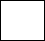
\includegraphics[height=1cm]{2_State_of_the_art/Arimaa_on_MCTS_Benoit/img/max.png}
		\caption{\label{fig:max}Nodes representing your moves are generally drawn as squares, these are also called MAX nodes.}
	\end{minipage}%
	\hspace*{1cm}
	\begin{minipage}[b]{0.45\linewidth}
		\centering
		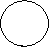
\includegraphics[height=1cm]{2_State_of_the_art/Arimaa_on_MCTS_Benoit/img/min.png}
		\caption{\label{fig:min}Nodes representing your opponent's moves are generally drawn as circles, these are also called MIN nodes.}
	\end{minipage}%
\end{figure}
\noindent
The goal at a MAX/MIN node is to maximize/minimize the value of the subtree rooted at that node. To do this, a MAX/MIN node chooses the child with the greatest/smallest value, and that becomes the value of the MAX/MIN node.\\
Note that it's typical for two player games to have different branching factors at each node. The move I make could make restrictions on what moves are possible for the other player, or possibly remove restrictions. Note also that in this example, we're ignoring what the game or the probem space are in order to focus on the algorithm.

\begin{figure}[H]
\centering
	\begin{minipage}[b]{0.45\linewidth}
		\centering
		\includegraphics[height=1.5cm]{2_State_of_the_art/Arimaa_on_MCTS_Benoit/img/Minimax2.png}
		\caption{\label{fig:Minimax2}When we start the problem, all Minimax sees is the start node.}
	\end{minipage}%
	\hspace*{1cm}
	\begin{minipage}[b]{0.45\linewidth}
		\centering
		\includegraphics[height=3cm]{2_State_of_the_art/Arimaa_on_MCTS_Benoit/img/Minimax3.png}
		\caption{\label{fig:Minimax3}It begins like a depth first search, generating the first child.}
	\end{minipage}%
\end{figure}

\noindent
So far we've really seen no evaluation values. The way Minimax works is to go down a specified number of full moves (where one ``full move'' is actually a move by you and a move by your opponent), then calculate evaluation values for states at that depth. For this example, we're going to go down one full move, which is one more level. 
\begin{figure}[H]
\centering
	\begin{minipage}[b]{0.45\linewidth}
		\centering
		\includegraphics[height=3cm]{2_State_of_the_art/Arimaa_on_MCTS_Benoit/img/Minimax4.png}
		\caption{\label{fig:Minimax4}we generate the values for those nodes.}
	\end{minipage}%
	\hspace*{1cm}
	\begin{minipage}[b]{0.45\linewidth}
		\centering
		\includegraphics[height=3cm]{2_State_of_the_art/Arimaa_on_MCTS_Benoit/img/Minimax5.png}
		\caption{\label{fig:Minimax5}It chooses the minimum of the two child node values, which is 3.}
	\end{minipage}%
\end{figure}

\noindent
The max node at the top still has two other children nodes that we need to generate and search.

\begin{figure}[H]
\centering
	\begin{minipage}[b]{0.45\linewidth}
		\centering
		\includegraphics[height=3cm]{2_State_of_the_art/Arimaa_on_MCTS_Benoit/img/Minimax6.png}
		\caption{\label{fig:Minimax6}Since there is only one child, the min node must take it's value.}
		\end{minipage}%
	\hspace*{1cm}
	\begin{minipage}[b]{0.45\linewidth}
		\centering
		\includegraphics[height=3cm]{2_State_of_the_art/Arimaa_on_MCTS_Benoit/img/Minimax8.png}
		\caption{\label{fig:Minimax8}The third min node chooses the minimum of it's child node values, 1.}
	\end{minipage}%
\end{figure}

\noindent
Finally we have all of the values of the children of the max node at the top level, so it chooses the maximum of them, 15, and we get the final solution. 

\begin{figure}[H]
\centering
	\begin{minipage}[b]{1\linewidth}
		\centering
		\includegraphics[height=3cm]{2_State_of_the_art/Arimaa_on_MCTS_Benoit/img/Minimax9.png}
		\caption{\label{fig:Minimax9}Final tree.}
	\end{minipage}%
\end{figure}

\noindent
What this tells us is that we should take the move that leads to the middle min node, since it'll lead to the best possible state for us one full move down the road. 

\subsection{The \ensuremath{\alpha\beta} pruning} %pruning = elaguage en anglais
The \ensuremath{\alpha\beta} method is a heuristic that decrease the number of leaf that will be explored by the Minimax algorithm. That way, the size of the tree will be smaller, the algorithm will be able to dive further and the time spend on more interesting subtree is greater.\\
If the leaf's position is less interesting than its parents, the algorithm won't explore anyfurther.

\subsection{Monte Carlo Tree Search Algorithm}
\subsubsection{Introduction}
Monte Carlo Tree Search (MCTS) is an algorithm used for making optimal decisions in Artificial Intelligence (AI) problems such as solving games or decision making in project managment. It is based on making a big number of random simulations in order to get trustfull datas. To make such simulations, the program play the moves randomly for each players. Once it reach a conclusion (win or loss), the program compute the statistics to get the odds of winning.
\subsubsection{How does it works ?}
The Algorithm create a tree with all possible solution with a small depth.
Then it start to run random simulations starting from the leaves in order to test the odds of the outcome.
Once we got enough the results (usually we are using time based simulations) we feed back the results and make the decision depending on the odds of each subsequent leaves.
\subsubsection{Example}
\label{sec:example}
\begin{figure}[H]
\centering
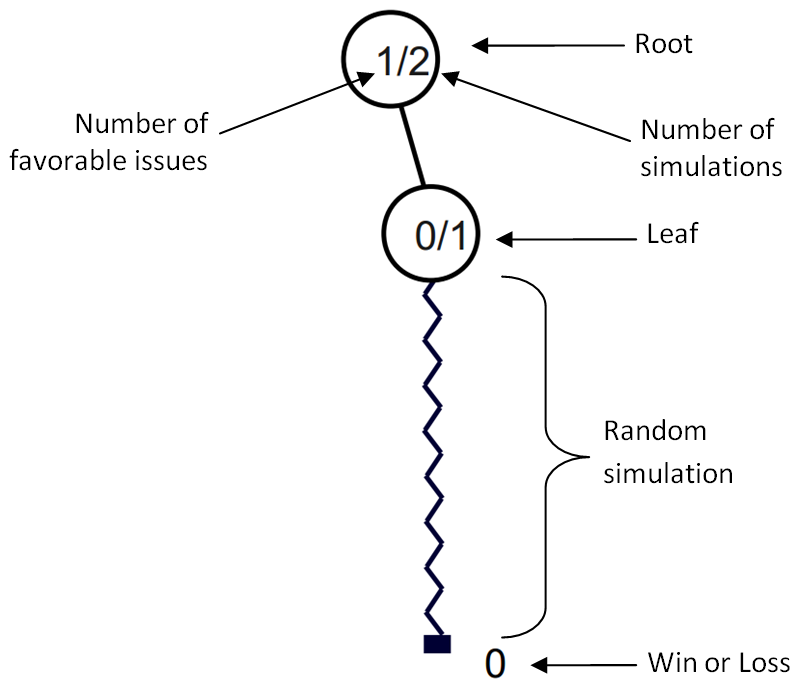
\includegraphics[height=5cm]{1_Presentation/1.2_Algorithm_MCTS_Benoit/img/schema.png}
\caption{\label{fig:schema}Legend of the following figures.}
\end{figure}

\begin{figure}[H]
\centering
	\begin{minipage}[b]{0.45\linewidth}
		\centering
		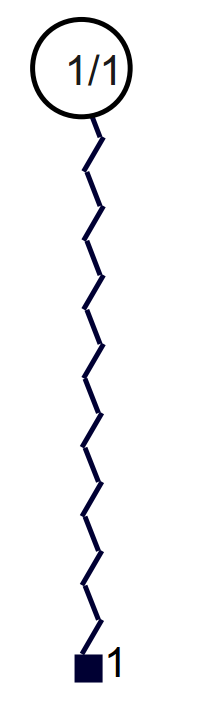
\includegraphics[height=4cm]{1_Presentation/1.2_Algorithm_MCTS_Benoit/img/1.png}
		\caption{\label{fig:1}Run a first simulation from the root, get a favorable issue (will be considered as a \textit{win}).}
	\end{minipage}%
	\hspace*{1cm}
	\begin{minipage}[b]{0.45\linewidth}
		\centering
		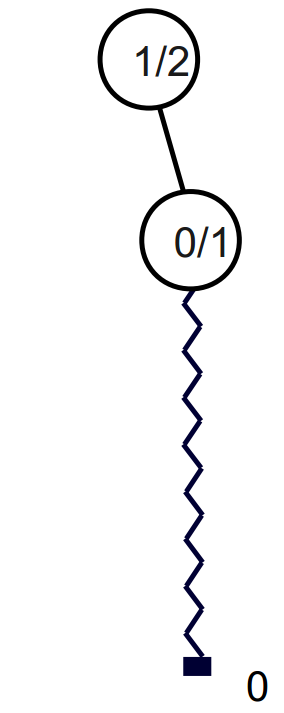
\includegraphics[height=4cm]{1_Presentation/1.2_Algorithm_MCTS_Benoit/img/2.png}
		\caption{\label{fig:2}Create a first leaf at depth 1 and run the simulation, get an unfavorable issue (considered as a \textit{loss}).}
	\end{minipage}%
\end{figure}

\begin{figure}[H]
\centering
	\begin{minipage}[b]{0.3\linewidth}
		\centering
		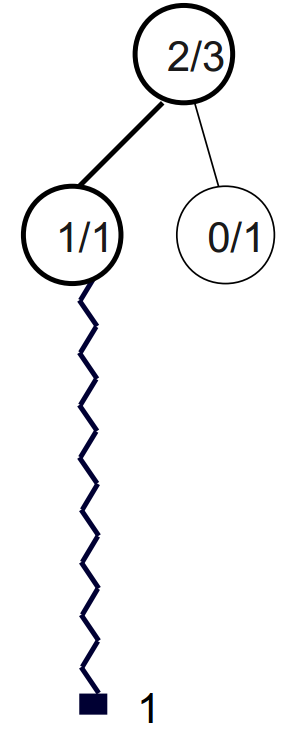
\includegraphics[height=4cm]{1_Presentation/1.2_Algorithm_MCTS_Benoit/img/3.png}
		\caption{\label{fig:3}Create a second leaf at depth 1 and run the simulation (\textit{win}).}
	\end{minipage}%
	\hspace*{1cm}
	\begin{minipage}[b]{0.3\linewidth}
		\centering
		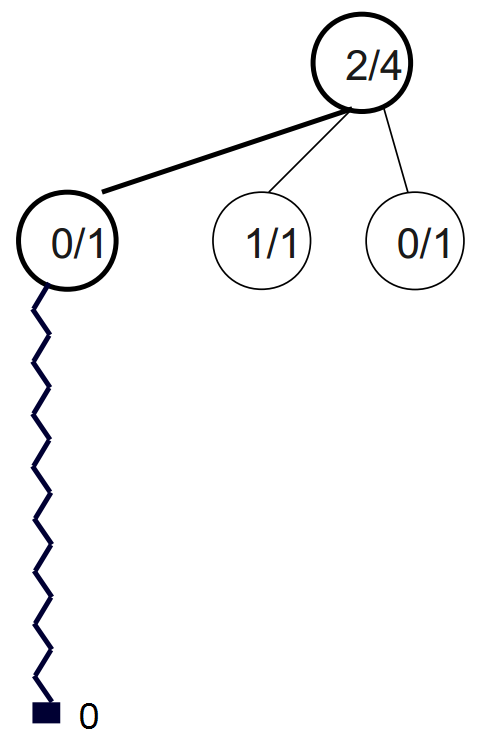
\includegraphics[height=4cm]{1_Presentation/1.2_Algorithm_MCTS_Benoit/img/4.png}
		\caption{\label{fig:4}Create a third leaf at depth 1 and run the simulation (\textit{loss}).}
	\end{minipage}%
	\hspace*{1cm}
	\begin{minipage}[b]{0.3\linewidth}
		\centering
		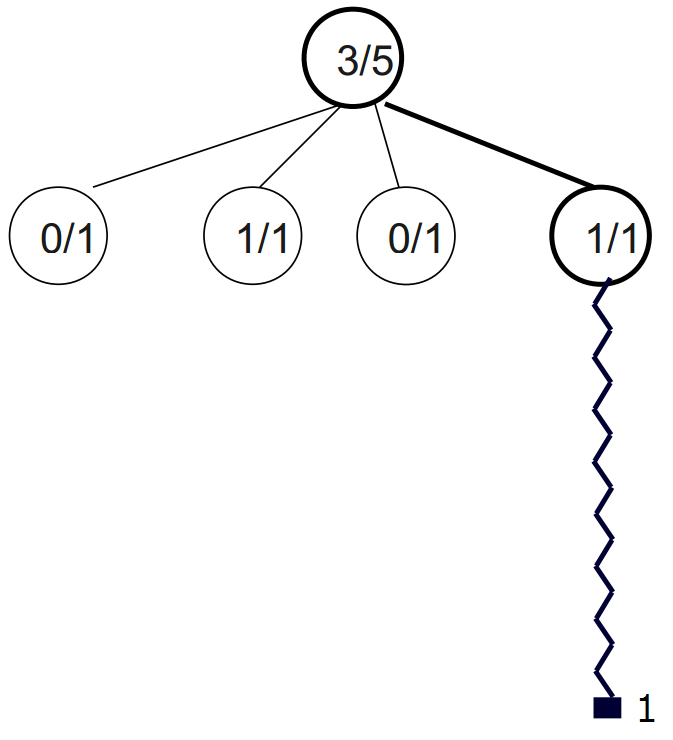
\includegraphics[height=4cm]{1_Presentation/1.2_Algorithm_MCTS_Benoit/img/5.png}
		\caption{\label{fig:5}Create a fourth leaf at depth 1 and run the simulation (\textit{win}).}
	\end{minipage}%
\end{figure}

\noindent
Right now the odds of winning are 3/5. Now that we tested all the possible outcomes at depth 1, we will expend the tree on the favorable leaves (here the second and fourth).

\begin{figure}[H]
\centering
	\begin{minipage}[b]{0.45\linewidth}
		\centering
		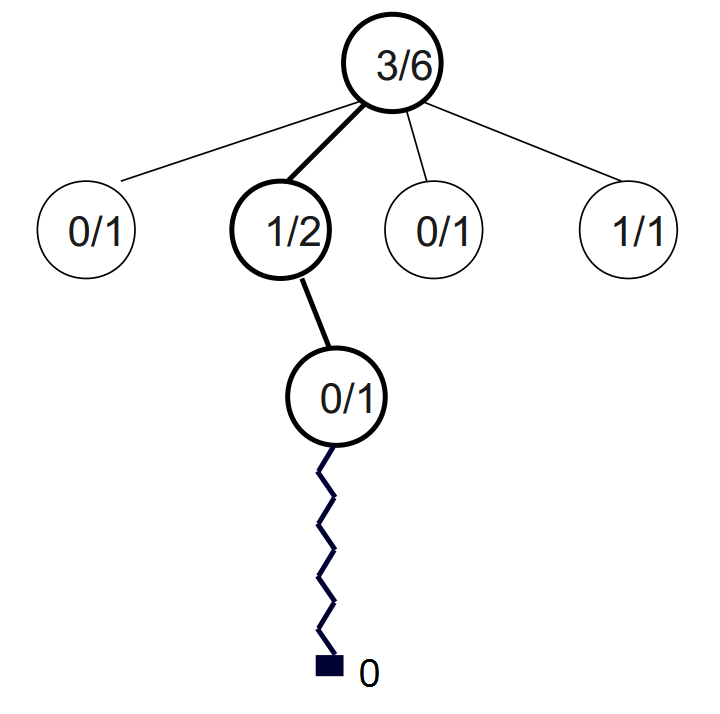
\includegraphics[height=4cm]{1_Presentation/1.2_Algorithm_MCTS_Benoit/img/6.png}
		\caption{\label{fig:6}Create a leaf at depth 2 with parent the 2nd leaf at depth 1 and run the simulation (\textit{loss}), update the odds value of the node and making it less interesting than the fourth node. Therefore the algorithm will now work on the fourth node.}
	\end{minipage}%
	\hspace*{1cm}
	\begin{minipage}[b]{0.45\linewidth}
		\centering
		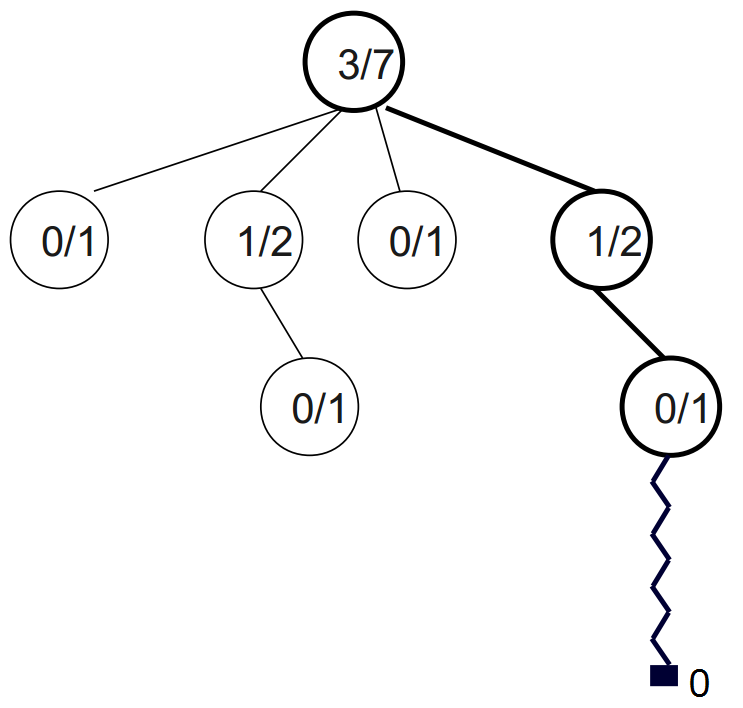
\includegraphics[height=4cm]{1_Presentation/1.2_Algorithm_MCTS_Benoit/img/7.png}
		\caption{\label{fig:7}Create a leaf at depth 2 with parent the fourth leaf at depth 1 and run the simulation (\textit{loss}), update the odds value of the node and making it as interesting as the second node. The algorithm will now work on the second node.}
	\end{minipage}%
\end{figure}
\begin{figure}[H]
\centering
	\begin{minipage}[b]{0.45\linewidth}
		\centering
		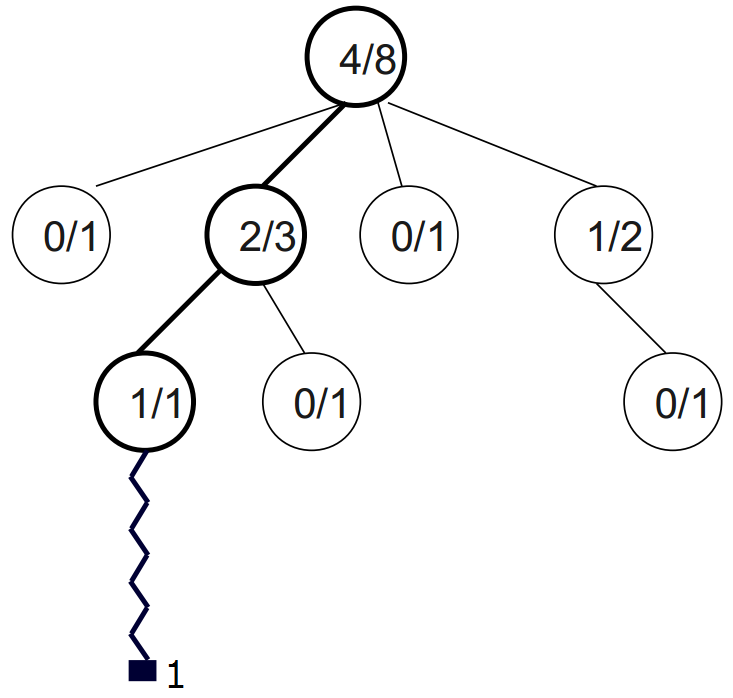
\includegraphics[height=4cm]{1_Presentation/1.2_Algorithm_MCTS_Benoit/img/8.png}
		\caption{\label{fig:8}Create a second leaf at depth 2 with parent the second leaf at depth 1 and run simulation (\textit{win}), update the odds value and continue to develop this leaf.}
	\end{minipage}%
	\hspace*{1cm}
	\begin{minipage}[b]{0.45\linewidth}
		\centering
		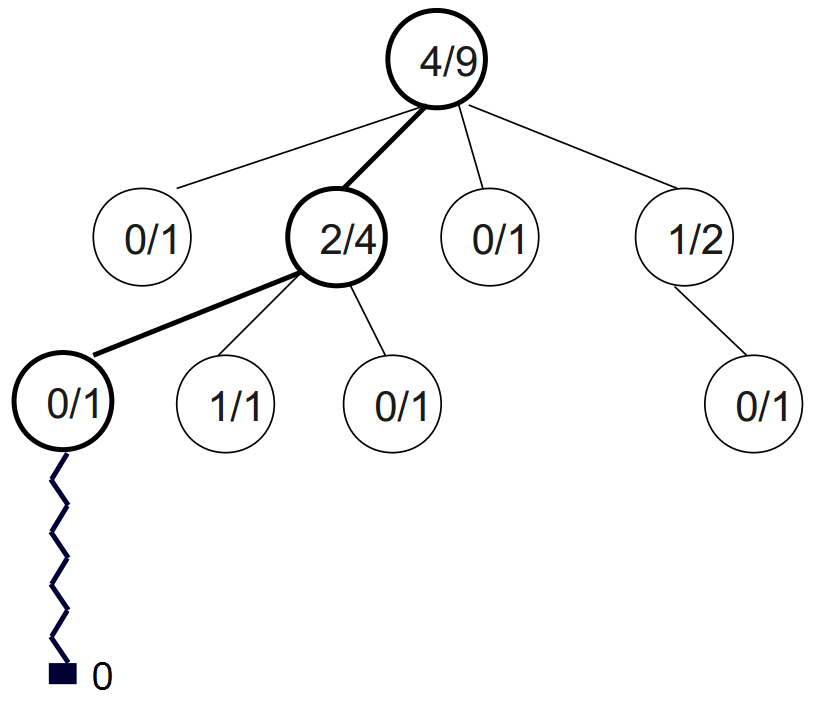
\includegraphics[height=4cm]{1_Presentation/1.2_Algorithm_MCTS_Benoit/img/9.png}
		\caption{\label{fig:9}Create a third leaf at depth 2 with parent the second leaf at depth 1 and run simulation (\textit{loss}), update the odds value and switch to the fourth leaf.}
	\end{minipage}%
\end{figure}
\noindent
Continue the Algorithm until a decent about of simulation are run and/or the time limit is .
\begin{figure}[H]
\centering
	\begin{minipage}[b]{0.33\linewidth}
	\centering
		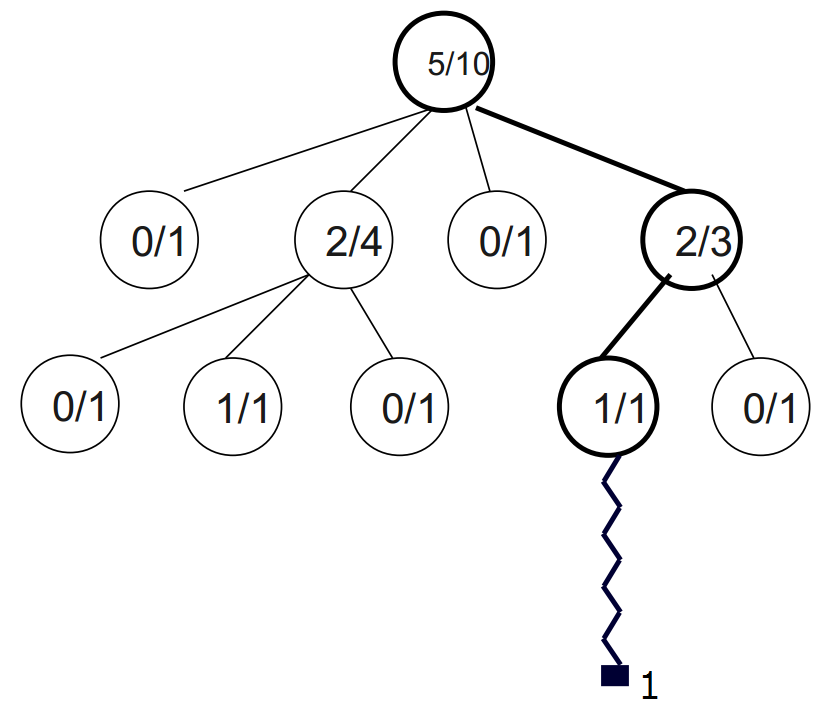
\includegraphics[height=4cm]{1_Presentation/1.2_Algorithm_MCTS_Benoit/img/10.png}
	\end{minipage}%
	\begin{minipage}[b]{0.33\linewidth}
	\centering
		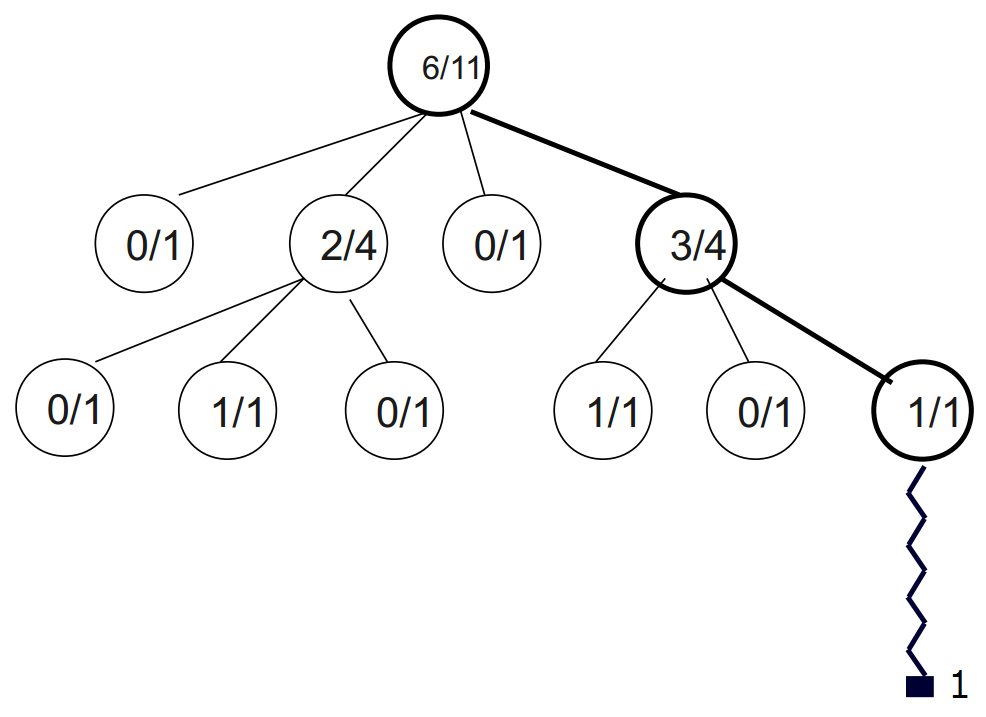
\includegraphics[height=4cm]{1_Presentation/1.2_Algorithm_MCTS_Benoit/img/11.png}
	\end{minipage}%
	\begin{minipage}[b]{0.33\linewidth}
	\centering
		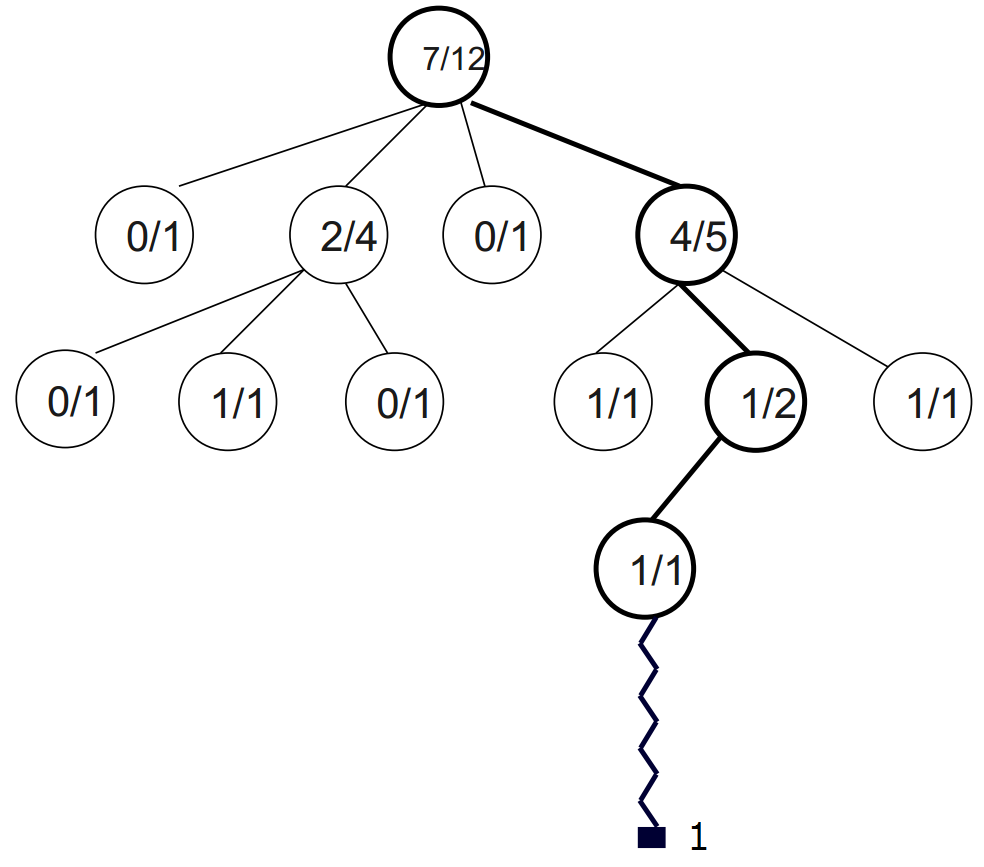
\includegraphics[height=4cm]{1_Presentation/1.2_Algorithm_MCTS_Benoit/img/12.png}
	\end{minipage}%
\end{figure}
\noindent
Make a decision : here we chose the fourth leaf.\\
\bigskip
\subsubsection{How to select the leaves to develop ?}
In the previous exemple, we chose to not expend leaves without winrates. But depending on the results of the simulations, wins can vary greatly. Therefore we will run more simulations on each leaf before chosing the ones to develop. For practical purpose we will select the leaves to expend that has the highest value of the cost function UCT (Upper Confidence Bound 1 applied to Trees).\\
\bigskip
\begin{minipage}[b]{1\linewidth}
\centering
\begin{equation*}
f = \frac{w_i}{n_i} + c\sqrt{\frac{\ln t}{n_i}}
\end{equation*}
\medskip
\textit{UCT function}\cite{formula_UCT}

\end{minipage}%
\bigskip
\begin{itemize}
  \item \ensuremath{w_i} : number of wins after the ith node
  \item \ensuremath{n_i} : number of simulations after the ith node
  \item \ensuremath{c}   : exploration parameter – theoretically equal to \ensuremath{\sqrt{2}} but in practice chosen empirically
  \item \ensuremath{t}   : total number of simulations in a given tree node, equal to the sum of all \ensuremath{n_i}
\end{itemize}
\medskip
The more a leaf is developed, the less it's cost is worth it. This way we can be sure that a leaf with low winrate isn't completely forgotten.\\

\subsubsection{Why using the Monte Carlo Tree Search ?}
Compared to other algorithm like Minimax, this one is generic, once you set the rules of the games, given enough time, it will solve it. The advantage of MCTS with it's basic form is that you don't need to implement functions to improve the researches. Based on its random simulations, it will determine by itself which are the good options and which aren't.\\ The more you run simulations, the more accurate the results will be.

\subsubsection{How much power do we need ?}
The more the game has possible moves, the more power it require to solve. In order to get plausible decisions, it needs to go deeper in the tree and to search enough leaves. If the time or number of simulations is not sufficient, the algorithm might miss some important branches and fail to give plausible results. Therefore in order to get decent results, using high-end computer is mandatory, it allows us to get access to multi-threading technology in order to parallelize the simulations.